% Options for packages loaded elsewhere
\PassOptionsToPackage{unicode}{hyperref}
\PassOptionsToPackage{hyphens}{url}
%
\documentclass[
]{article}
\usepackage{amsmath,amssymb}
\usepackage{iftex}
\ifPDFTeX
  \usepackage[T1]{fontenc}
  \usepackage[utf8]{inputenc}
  \usepackage{textcomp} % provide euro and other symbols
\else % if luatex or xetex
  \usepackage{unicode-math} % this also loads fontspec
  \defaultfontfeatures{Scale=MatchLowercase}
  \defaultfontfeatures[\rmfamily]{Ligatures=TeX,Scale=1}
\fi
\usepackage{lmodern}
\ifPDFTeX\else
  % xetex/luatex font selection
\fi
% Use upquote if available, for straight quotes in verbatim environments
\IfFileExists{upquote.sty}{\usepackage{upquote}}{}
\IfFileExists{microtype.sty}{% use microtype if available
  \usepackage[]{microtype}
  \UseMicrotypeSet[protrusion]{basicmath} % disable protrusion for tt fonts
}{}
\makeatletter
\@ifundefined{KOMAClassName}{% if non-KOMA class
  \IfFileExists{parskip.sty}{%
    \usepackage{parskip}
  }{% else
    \setlength{\parindent}{0pt}
    \setlength{\parskip}{6pt plus 2pt minus 1pt}}
}{% if KOMA class
  \KOMAoptions{parskip=half}}
\makeatother
\usepackage{xcolor}
\usepackage[margin=1in]{geometry}
\usepackage{listings}
\newcommand{\passthrough}[1]{#1}
\lstset{defaultdialect=[5.3]Lua}
\lstset{defaultdialect=[x86masm]Assembler}
\usepackage{graphicx}
\makeatletter
\def\maxwidth{\ifdim\Gin@nat@width>\linewidth\linewidth\else\Gin@nat@width\fi}
\def\maxheight{\ifdim\Gin@nat@height>\textheight\textheight\else\Gin@nat@height\fi}
\makeatother
% Scale images if necessary, so that they will not overflow the page
% margins by default, and it is still possible to overwrite the defaults
% using explicit options in \includegraphics[width, height, ...]{}
\setkeys{Gin}{width=\maxwidth,height=\maxheight,keepaspectratio}
% Set default figure placement to htbp
\makeatletter
\def\fps@figure{htbp}
\makeatother
\setlength{\emergencystretch}{3em} % prevent overfull lines
\providecommand{\tightlist}{%
  \setlength{\itemsep}{0pt}\setlength{\parskip}{0pt}}
\setcounter{secnumdepth}{-\maxdimen} % remove section numbering
\lstset{
	breaklines=true
}
\ifLuaTeX
  \usepackage{selnolig}  % disable illegal ligatures
\fi
\IfFileExists{bookmark.sty}{\usepackage{bookmark}}{\usepackage{hyperref}}
\IfFileExists{xurl.sty}{\usepackage{xurl}}{} % add URL line breaks if available
\urlstyle{same}
\hypersetup{
  pdftitle={Lab 1 Block 2 Report},
  pdfauthor={Marijn Jaarsma \& Simon Jorstedt \& Hugo Morvan},
  hidelinks,
  pdfcreator={LaTeX via pandoc}}

\title{Lab 1 Block 2 Report}
\author{Marijn Jaarsma \& Simon Jorstedt \& Hugo Morvan}
\date{2023-11-27}

\begin{document}
\maketitle

\hypertarget{ensemble-methods}{%
\section{1. Ensemble Methods}\label{ensemble-methods}}

Your task is to learn some random forests using the function
randomForest from the R package randomForest. The training data is
produced by running the following R code:

\begin{lstlisting}[language=R]
x1<-runif(100)
x2<-runif(100)
trdata<-cbind(x1,x2)
y<-as.numeric(x1<x2)
trlabels<-as.factor(y)
\end{lstlisting}

The task is therefore classifying Y from X1 and X2 , where Y is binary
and X1 and X2 continuous. You should learn a random forest with 1, 10
and 100 trees, which you can do by setting the argument ntree to the
appropriate value. Use nodesize = 25 and keep.forest = TRUE. The latter
saves the random forest learned. You need it because you should also
compute the misclassification error in the following test dataset (use
the function predict for this purpose):

\begin{lstlisting}[language=R]
set.seed(1234)
x1<-runif(1000)
x2<-runif(1000)
tedata<-cbind(x1,x2)
y<-as.numeric(x1<x2)
telabels<-as.factor(y)
plot(x1,x2,col=(y+1))
\end{lstlisting}

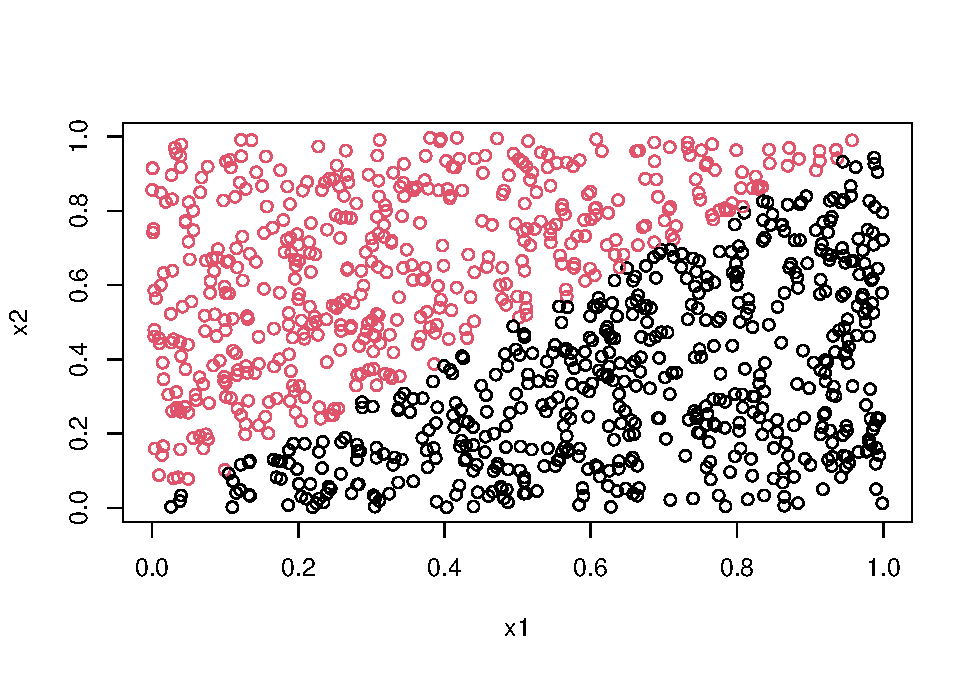
\includegraphics{Block2Lab1_files/figure-latex/1.1-1.pdf}

\begin{lstlisting}[language=R]
get_misc_err <- function(conf_mat){
  #Given a confusion matrix, return the misclassification error
  (sum(conf_mat)-sum(diag(conf_mat)))/sum(conf_mat)
}

r1 <- randomForest(trdata, trlabels, ntree = 1, nodesize = 25, keep.forest = TRUE)
p1 <- predict(r1, tedata)
conf_mat1 <- table(p1, telabels)
get_misc_err(conf_mat1)
\end{lstlisting}

\begin{lstlisting}
## [1] 0.206
\end{lstlisting}

\begin{lstlisting}[language=R]
cat("Mean misclassification error for 1 tree:", get_misc_err(conf_mat1), "\n")
\end{lstlisting}

\begin{lstlisting}
## Mean misclassification error for 1 tree: 0.206
\end{lstlisting}

\begin{lstlisting}[language=R]
r10 <- randomForest(trdata, trlabels, ntree = 10, nodesize = 25, keep.forest = TRUE)
p10 <- predict(r10, tedata)
conf_mat10 <- table(p10, telabels)
get_misc_err(conf_mat10)
\end{lstlisting}

\begin{lstlisting}
## [1] 0.106
\end{lstlisting}

\begin{lstlisting}[language=R]
cat("Mean misclassification error for 10 trees:", get_misc_err(conf_mat10), "\n")
\end{lstlisting}

\begin{lstlisting}
## Mean misclassification error for 10 trees: 0.106
\end{lstlisting}

\begin{lstlisting}[language=R]
r100 <- randomForest(trdata, trlabels, ntree = 100, nodesize = 25, keep.forest = TRUE)
p100 <- predict(r100, tedata)
conf_mat100 <- table(p100, telabels)
get_misc_err(conf_mat100)
\end{lstlisting}

\begin{lstlisting}
## [1] 0.07
\end{lstlisting}

\begin{lstlisting}[language=R]
cat("Mean misclassification error for 100 trees:", get_misc_err(conf_mat100), "\n")
\end{lstlisting}

\begin{lstlisting}
## Mean misclassification error for 100 trees: 0.07
\end{lstlisting}

Repeat the procedure above for 1000 training datasets of size 100 and
report the mean and variance of the misclassification errors. In other
words, create 1000 training datasets of size 100, learn a random forest
from each dataset, and compute the misclassification error in the same
test dataset of size 1000. Report results for when the random forest has
1, 10 and 100 trees.

\begin{lstlisting}[language=R]
get_training <- function(){
  x1<-runif(100)
  x2<-runif(100)
  trdata<-cbind(x1,x2)
  y<-as.numeric(x1<x2)
  trlabels<-as.factor(y)
  return(list(trdata, trlabels))
}
meR1 <- c()

meR10 <- c()

meR100 <- c()

for(i in 1:1000){
  
  #cat("Iteration:", i, "\r")
  #Creating the training data
  training <- get_training()
  trdata <- training[[1]]
  trlabels <- training[[2]]
  
  
  r1 <- randomForest(trdata, trlabels, ntree = 1, nodesize = 25, keep.forest = TRUE)
  p1 <- predict(r1, tedata)
  conf_mat1 <- table(p1, telabels)
  meR1 <- c(meR1, get_misc_err(conf_mat1))
  
  r10 <- randomForest(trdata, trlabels, ntree = 10, nodesize = 25, keep.forest = TRUE)
  p10 <- predict(r10, tedata)
  conf_mat10 <- table(p10, telabels)
  meR10 <- c(meR10, get_misc_err(conf_mat10))
  
  r100 <- randomForest(trdata, trlabels, ntree = 100, nodesize = 25, keep.forest = TRUE)
  p100 <- predict(r100, tedata)
  conf_mat100 <- table(p100, telabels)
  meR100 <- c(meR100, get_misc_err(conf_mat100))
}

#Overall mean
cat("Overall mean for 1 tree:", mean(meR1), "\n")
\end{lstlisting}

\begin{lstlisting}
## Overall mean for 1 tree: 0.209284
\end{lstlisting}

\begin{lstlisting}[language=R]
cat("Overall variance for 1 tree:", var(meR1), "\n")
\end{lstlisting}

\begin{lstlisting}
## Overall variance for 1 tree: 0.00309292
\end{lstlisting}

\begin{lstlisting}[language=R]
cat("Overall mean for 10 trees:", mean(meR10), "\n")
\end{lstlisting}

\begin{lstlisting}
## Overall mean for 10 trees: 0.134774
\end{lstlisting}

\begin{lstlisting}[language=R]
cat("Overall variance for 10 trees:", var(meR10), "\n")
\end{lstlisting}

\begin{lstlisting}
## Overall variance for 10 trees: 0.0008590079
\end{lstlisting}

\begin{lstlisting}[language=R]
cat("Overall mean for 100 trees:", mean(meR100), "\n")
\end{lstlisting}

\begin{lstlisting}
## Overall mean for 100 trees: 0.111006
\end{lstlisting}

\begin{lstlisting}[language=R]
cat("Overall variance for 100 trees:", var(meR100), "\n")
\end{lstlisting}

\begin{lstlisting}
## Overall variance for 100 trees: 0.0008635495
\end{lstlisting}

Repeat the exercise above but this time use the condition
(x1\textless0.5) instead of (x1\textless x2) when producing the training
and test datasets.

\begin{lstlisting}[language=R]
set.seed(1234)
x1<-runif(1000)
x2<-runif(1000)
tedata<-cbind(x1,x2)
y<-as.numeric(x1<0.5)
telabels<-as.factor(y)
plot(x1,x2,col=(y+1))
\end{lstlisting}

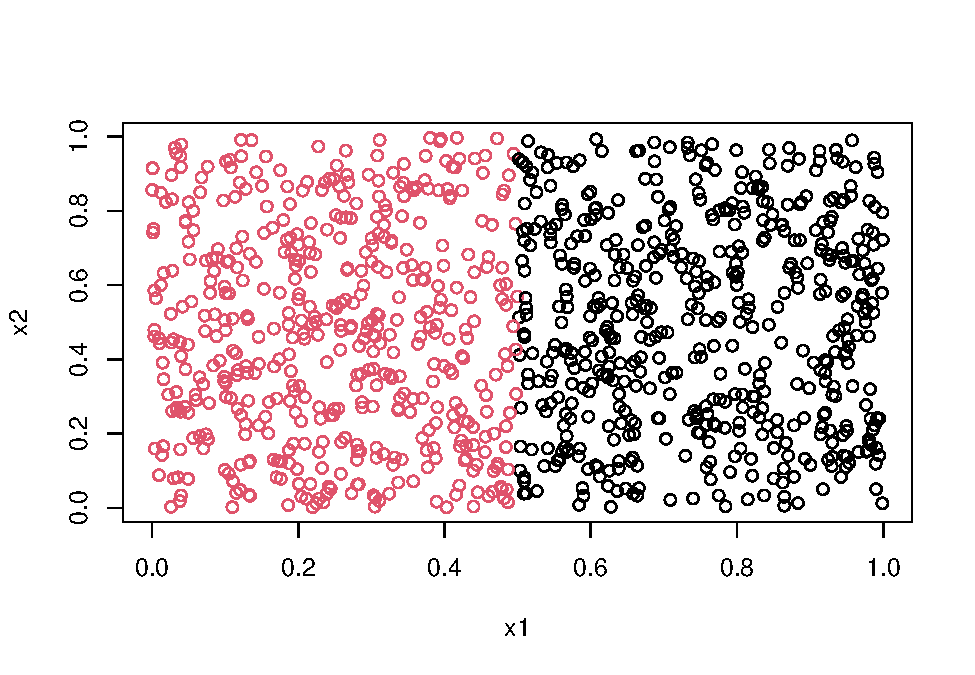
\includegraphics{Block2Lab1_files/figure-latex/1.3-1.pdf}

\begin{lstlisting}[language=R]
get_training <- function(){
  x1<-runif(100)
  x2<-runif(100)
  trdata<-cbind(x1,x2)
  y<-as.numeric(x1<0.5)
  trlabels<-as.factor(y)
  return(list(trdata, trlabels))
}
meR1 <- c()

meR10 <- c()

meR100 <- c()

for(i in 1:1000){
  
  #cat("Iteration:", i, "\r")
  #Creating the training data
  training <- get_training()
  trdata <- training[[1]]
  trlabels <- training[[2]]
  
  
  r1 <- randomForest(trdata, trlabels, ntree = 1, nodesize = 25, keep.forest = TRUE)
  p1 <- predict(r1, tedata)
  conf_mat1 <- table(p1, telabels)
  meR1 <- c(meR1, get_misc_err(conf_mat1))
  
  r10 <- randomForest(trdata, trlabels, ntree = 10, nodesize = 25, keep.forest = TRUE)
  p10 <- predict(r10, tedata)
  conf_mat10 <- table(p10, telabels)
  meR10 <- c(meR10, get_misc_err(conf_mat10))
  
  r100 <- randomForest(trdata, trlabels, ntree = 100, nodesize = 25, keep.forest = TRUE)
  p100 <- predict(r100, tedata)
  conf_mat100 <- table(p100, telabels)
  meR100 <- c(meR100, get_misc_err(conf_mat100))
}

#Overall mean
cat("Overall mean for 1 tree:", mean(meR1), "\n")
\end{lstlisting}

\begin{lstlisting}
## Overall mean for 1 tree: 0.092951
\end{lstlisting}

\begin{lstlisting}[language=R]
cat("Overall variance for 1 tree:", var(meR1), "\n")
\end{lstlisting}

\begin{lstlisting}
## Overall variance for 1 tree: 0.01729452
\end{lstlisting}

\begin{lstlisting}[language=R]
cat("Overall mean for 10 trees:", mean(meR10), "\n")
\end{lstlisting}

\begin{lstlisting}
## Overall mean for 10 trees: 0.013772
\end{lstlisting}

\begin{lstlisting}[language=R]
cat("Overall variance for 10 trees:", var(meR10), "\n")
\end{lstlisting}

\begin{lstlisting}
## Overall variance for 10 trees: 0.0004568148
\end{lstlisting}

\begin{lstlisting}[language=R]
cat("Overall mean for 100 trees:", mean(meR100), "\n")
\end{lstlisting}

\begin{lstlisting}
## Overall mean for 100 trees: 0.006414
\end{lstlisting}

\begin{lstlisting}[language=R]
cat("Overall variance for 100 trees:", var(meR100), "\n")
\end{lstlisting}

\begin{lstlisting}
## Overall variance for 100 trees: 6.676737e-05
\end{lstlisting}

Repeat the exercise above but this time use the condition
((x1\textless0.5 \& x2\textless0.5) \textbar{} (x1\textgreater0.5 \&
x2\textgreater0.5)) instead of (x1\textless x2) when producing the
training and test datasets. Unlike above, use nodesize = 12 for this
exercise.

\begin{lstlisting}[language=R]
set.seed(1234)
x1<-runif(1000)
x2<-runif(1000)
tedata<-cbind(x1,x2)
y<-as.numeric(((x1<0.5 & x2<0.5) | (x1>0.5 & x2>0.5)))
telabels<-as.factor(y)
plot(x1,x2,col=(y+1))
\end{lstlisting}

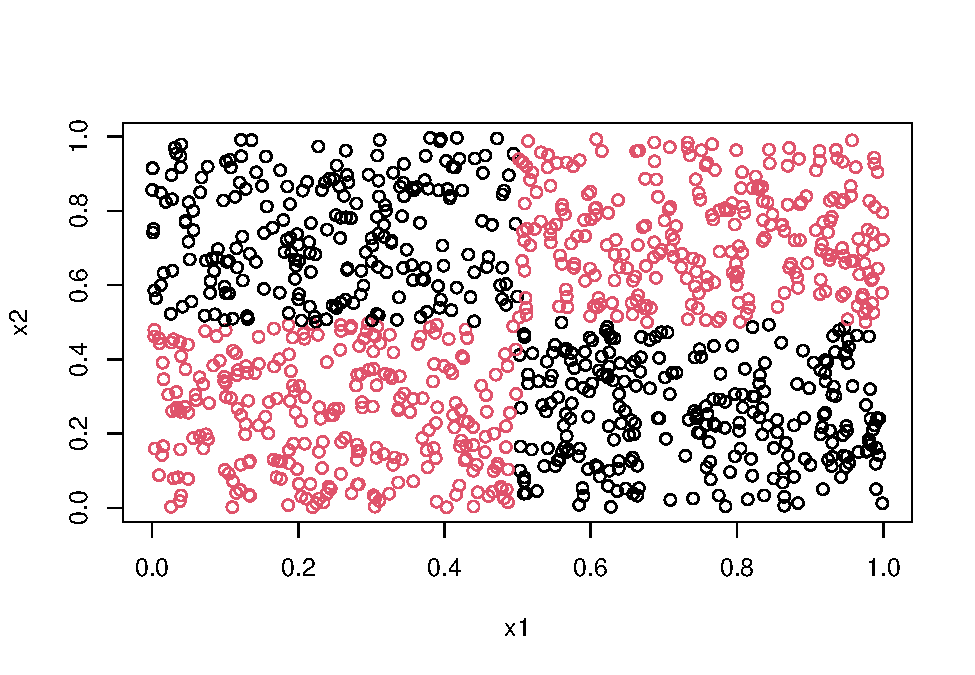
\includegraphics{Block2Lab1_files/figure-latex/1.4-1.pdf}

\begin{lstlisting}[language=R]
get_training <- function(){
  x1<-runif(100)
  x2<-runif(100)
  trdata<-cbind(x1,x2)
  y<-as.numeric((x1<0.5 & x2<0.5) | (x1>0.5 & x2>0.5))
  trlabels<-as.factor(y)
  return(list(trdata, trlabels))
}
meR1 <- c()

meR10 <- c()

meR100 <- c()

for(i in 1:1000){
  
  #cat("Iteration:", i, "\r")
  #Creating the training data
  training <- get_training()
  trdata <- training[[1]]
  trlabels <- training[[2]]
  
  
  r1 <- randomForest(trdata, trlabels, ntree = 1, nodesize = 12, keep.forest = TRUE)
  p1 <- predict(r1, tedata)
  conf_mat1 <- table(p1, telabels)
  meR1 <- c(meR1, get_misc_err(conf_mat1))
  
  r10 <- randomForest(trdata, trlabels, ntree = 10, nodesize = 12, keep.forest = TRUE)
  p10 <- predict(r10, tedata)
  conf_mat10 <- table(p10, telabels)
  meR10 <- c(meR10, get_misc_err(conf_mat10))
  
  r100 <- randomForest(trdata, trlabels, ntree = 100, nodesize = 12, keep.forest = TRUE)
  p100 <- predict(r100, tedata)
  conf_mat100 <- table(p100, telabels)
  meR100 <- c(meR100, get_misc_err(conf_mat100))
}

#Overall mean
cat("Overall mean for 1 tree:", mean(meR1), "\n")
\end{lstlisting}

\begin{lstlisting}
## Overall mean for 1 tree: 0.251183
\end{lstlisting}

\begin{lstlisting}[language=R]
cat("Overall variance for 1 tree:", var(meR1), "\n")
\end{lstlisting}

\begin{lstlisting}
## Overall variance for 1 tree: 0.01325594
\end{lstlisting}

\begin{lstlisting}[language=R]
cat("Overall mean for 10 trees:", mean(meR10), "\n")
\end{lstlisting}

\begin{lstlisting}
## Overall mean for 10 trees: 0.122827
\end{lstlisting}

\begin{lstlisting}[language=R]
cat("Overall variance for 10 trees:", var(meR10), "\n")
\end{lstlisting}

\begin{lstlisting}
## Overall variance for 10 trees: 0.00320077
\end{lstlisting}

\begin{lstlisting}[language=R]
cat("Overall mean for 100 trees:", mean(meR100), "\n")
\end{lstlisting}

\begin{lstlisting}
## Overall mean for 100 trees: 0.076979
\end{lstlisting}

\begin{lstlisting}[language=R]
cat("Overall variance for 100 trees:", var(meR100), "\n")
\end{lstlisting}

\begin{lstlisting}
## Overall variance for 100 trees: 0.001413212
\end{lstlisting}

Answer the following questions: -- What happens with the mean error rate
when the number of trees in the random forest grows? Why?

The mean error rate decreases as the number of trees in the random
forest grows. This is because as the number of tree increases, the
``wisdom of crowd'' effect intensifies

-- The third dataset represents a slightly more complicated
classification problem than the first one. Still, you should get better
performance for it when using sufficient trees in the random forest.
Explain why you get better performance.

We still get better performances because as the number of trees
increases, we reduce the chances of overfitting by having many different
trees that ignores the random variation in the training data and also
reduces the variance of the ensemble model.

\hypertarget{mixture-models}{%
\section{2. Mixture Models}\label{mixture-models}}

Your task is to implement the EM algorithm for Bernoulli mixture model.
Please use the R template below to solve the assignment. Then, use your
implementation to show what happens when your mixture model has too few
and too many clusters, i.e.~set M = 2, 3, 4 and compare results. Please
provide a short explanation as well. A Bernoulli mixture model is
\[p(x) = \sum_{m=1}^{M}{\pi_m Bern(x|\mu_m)}\] where
\(x = (x_1,...,x_D)\) is a D-dimensional binary random vector,
\(\pi_m = p(y = m)\) and
\[Bern(x|\mu_m) = \prod_{d=1}^{D}{\mu_{m,d}^{x_d}(1-\mu_{m,d})^{(1-x_d)} }\]

where \(\mu_m = (\mu_{m,1} , . . . , \mu_{m,D} )\) is a D-dimensional
vector of probabilities. As usual, the log likelihood of the dataset
\(\begin{Bmatrix}x_i\end{Bmatrix}_{i=1}^{n}\) is
\[\sum_{i=1}^{M}\log p(x_i)\]

Finally, in the EM algorithm, the parameter updates for the Bernoulli
mixture model are the same as for the Gaussian mixture model (see
Equations 10.16a,b in the lecture slides).

\begin{lstlisting}[language=R]
set.seed(1234567890)
max_it <- 100 # max number of EM iterations
min_change <- 0.1 # min change in log lik between two consecutive iterations
n=1000 # number of training points
D=10 # number of dimensions
x <- matrix(nrow=n, ncol=D) # training data
true_pi <- vector(length = 3) # true mixing coefficients
true_mu <- matrix(nrow=3, ncol=D) # true conditional distributions
true_pi=c(1/3, 1/3, 1/3)
true_mu[1,]=c(0.5,0.6,0.4,0.7,0.3,0.8,0.2,0.9,0.1,1)
true_mu[2,]=c(0.5,0.4,0.6,0.3,0.7,0.2,0.8,0.1,0.9,0)
true_mu[3,]=c(0.5,0.5,0.5,0.5,0.5,0.5,0.5,0.5,0.5,0.5)
plot(true_mu[1,], type="o", col="blue", ylim=c(0,1))
points(true_mu[2,], type="o", col="red")
points(true_mu[3,], type="o", col="green")
\end{lstlisting}

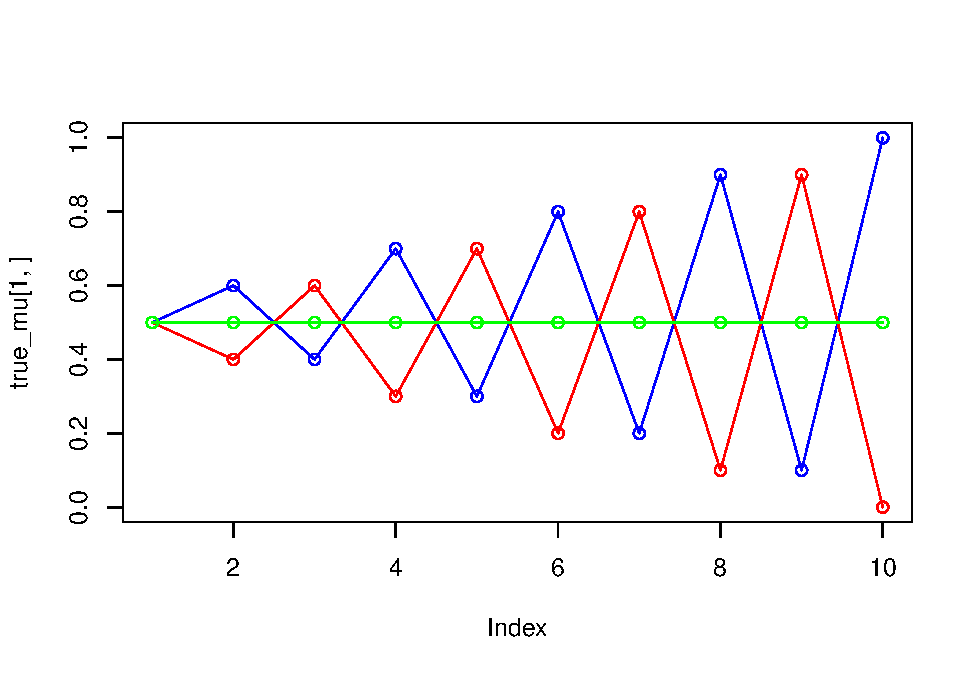
\includegraphics{Block2Lab1_files/figure-latex/2.1-1.pdf}

\begin{lstlisting}[language=R]
# Producing the training data
for(i in 1:n){
  m <- sample(1:3,1,prob=true_pi)
  for(d in 1:D){
    x[i,d] <- rbinom(1,1,true_mu[m,d])
  }
}
M=3 # number of clusters
w <- matrix(nrow=n, ncol=M) # weights
pi <- vector(length = M) # mixing coefficients
mu <- matrix(nrow=M, ncol=D) # conditional distributions
llik <- vector(length = max_it) # log likelihood of the EM iterations
# Random initialization of the parameters
pi <- runif(M,0.49,0.51)
pi <- pi / sum(pi)
for(m in 1:M){
  mu[m,] <- runif(D,0.49,0.51)
}
pi
\end{lstlisting}

\begin{lstlisting}
## [1] 0.3326090 0.3336558 0.3337352
\end{lstlisting}

\begin{lstlisting}[language=R]
mu
\end{lstlisting}

\begin{lstlisting}
##           [,1]      [,2]      [,3]      [,4]      [,5]      [,6]      [,7]
## [1,] 0.4939877 0.4935375 0.5042511 0.5040286 0.4987810 0.5012754 0.4971036
## [2,] 0.4993719 0.5088453 0.5068730 0.5016720 0.4929275 0.5077146 0.5095075
## [3,] 0.4975302 0.5077926 0.4939841 0.5059821 0.5063490 0.5041462 0.4929400
##           [,8]      [,9]     [,10]
## [1,] 0.4982144 0.4987654 0.4929075
## [2,] 0.4924574 0.4992470 0.5008651
## [3,] 0.4992362 0.4943482 0.4903974
\end{lstlisting}

\begin{lstlisting}[language=R]
for(it in 1:max_it) {
  plot(mu[1,], type="o", col="blue", ylim=c(0,1))
  points(mu[2,], type="o", col="red")
  points(mu[3,], type="o", col="green")
  #points(mu[4,], type="o", col="yellow")
  Sys.sleep(0.1)
  # E-step: Computation of the weights
  # Your code here
  #Log likelihood computation.
  # Your code here
  cat("iteration: ", it, "log likelihood: ", llik[it], "\n")
  flush.console()
  # Stop if the lok likelihood has not changed significantly
  # Your code here
  #M-step: ML parameter estimation from the data and weights
  # Your code here
}
\end{lstlisting}

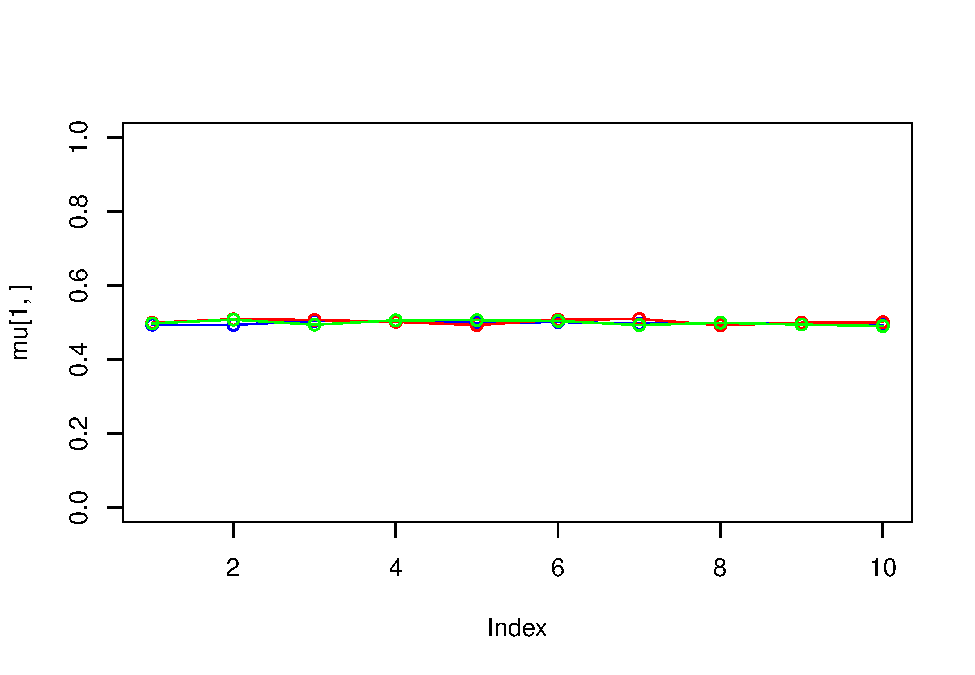
\includegraphics{Block2Lab1_files/figure-latex/2.1-2.pdf}

\begin{lstlisting}
## iteration:  1 log likelihood:  FALSE
\end{lstlisting}

\begin{lstlisting}
## iteration:  2 log likelihood:  FALSE
\end{lstlisting}

\begin{lstlisting}
## iteration:  3 log likelihood:  FALSE
\end{lstlisting}

\begin{lstlisting}
## iteration:  4 log likelihood:  FALSE
\end{lstlisting}

\begin{lstlisting}
## iteration:  5 log likelihood:  FALSE
\end{lstlisting}

\begin{lstlisting}
## iteration:  6 log likelihood:  FALSE
\end{lstlisting}

\begin{lstlisting}
## iteration:  7 log likelihood:  FALSE
\end{lstlisting}

\begin{lstlisting}
## iteration:  8 log likelihood:  FALSE
\end{lstlisting}

\begin{lstlisting}
## iteration:  9 log likelihood:  FALSE
\end{lstlisting}

\begin{lstlisting}
## iteration:  10 log likelihood:  FALSE
\end{lstlisting}

\begin{lstlisting}
## iteration:  11 log likelihood:  FALSE
\end{lstlisting}

\begin{lstlisting}
## iteration:  12 log likelihood:  FALSE
\end{lstlisting}

\begin{lstlisting}
## iteration:  13 log likelihood:  FALSE
\end{lstlisting}

\begin{lstlisting}
## iteration:  14 log likelihood:  FALSE
\end{lstlisting}

\begin{lstlisting}
## iteration:  15 log likelihood:  FALSE
\end{lstlisting}

\begin{lstlisting}
## iteration:  16 log likelihood:  FALSE
\end{lstlisting}

\begin{lstlisting}
## iteration:  17 log likelihood:  FALSE
\end{lstlisting}

\begin{lstlisting}
## iteration:  18 log likelihood:  FALSE
\end{lstlisting}

\begin{lstlisting}
## iteration:  19 log likelihood:  FALSE
\end{lstlisting}

\begin{lstlisting}
## iteration:  20 log likelihood:  FALSE
\end{lstlisting}

\begin{lstlisting}
## iteration:  21 log likelihood:  FALSE
\end{lstlisting}

\begin{lstlisting}
## iteration:  22 log likelihood:  FALSE
\end{lstlisting}

\begin{lstlisting}
## iteration:  23 log likelihood:  FALSE
\end{lstlisting}

\begin{lstlisting}
## iteration:  24 log likelihood:  FALSE
\end{lstlisting}

\begin{lstlisting}
## iteration:  25 log likelihood:  FALSE
\end{lstlisting}

\begin{lstlisting}
## iteration:  26 log likelihood:  FALSE
\end{lstlisting}

\begin{lstlisting}
## iteration:  27 log likelihood:  FALSE
\end{lstlisting}

\begin{lstlisting}
## iteration:  28 log likelihood:  FALSE
\end{lstlisting}

\begin{lstlisting}
## iteration:  29 log likelihood:  FALSE
\end{lstlisting}

\begin{lstlisting}
## iteration:  30 log likelihood:  FALSE
\end{lstlisting}

\begin{lstlisting}
## iteration:  31 log likelihood:  FALSE
\end{lstlisting}

\begin{lstlisting}
## iteration:  32 log likelihood:  FALSE
\end{lstlisting}

\begin{lstlisting}
## iteration:  33 log likelihood:  FALSE
\end{lstlisting}

\begin{lstlisting}
## iteration:  34 log likelihood:  FALSE
\end{lstlisting}

\begin{lstlisting}
## iteration:  35 log likelihood:  FALSE
\end{lstlisting}

\begin{lstlisting}
## iteration:  36 log likelihood:  FALSE
\end{lstlisting}

\begin{lstlisting}
## iteration:  37 log likelihood:  FALSE
\end{lstlisting}

\begin{lstlisting}
## iteration:  38 log likelihood:  FALSE
\end{lstlisting}

\begin{lstlisting}
## iteration:  39 log likelihood:  FALSE
\end{lstlisting}

\begin{lstlisting}
## iteration:  40 log likelihood:  FALSE
\end{lstlisting}

\begin{lstlisting}
## iteration:  41 log likelihood:  FALSE
\end{lstlisting}

\begin{lstlisting}
## iteration:  42 log likelihood:  FALSE
\end{lstlisting}

\begin{lstlisting}
## iteration:  43 log likelihood:  FALSE
\end{lstlisting}

\begin{lstlisting}
## iteration:  44 log likelihood:  FALSE
\end{lstlisting}

\begin{lstlisting}
## iteration:  45 log likelihood:  FALSE
\end{lstlisting}

\begin{lstlisting}
## iteration:  46 log likelihood:  FALSE
\end{lstlisting}

\begin{lstlisting}
## iteration:  47 log likelihood:  FALSE
\end{lstlisting}

\begin{lstlisting}
## iteration:  48 log likelihood:  FALSE
\end{lstlisting}

\begin{lstlisting}
## iteration:  49 log likelihood:  FALSE
\end{lstlisting}

\begin{lstlisting}
## iteration:  50 log likelihood:  FALSE
\end{lstlisting}

\begin{lstlisting}
## iteration:  51 log likelihood:  FALSE
\end{lstlisting}

\begin{lstlisting}
## iteration:  52 log likelihood:  FALSE
\end{lstlisting}

\begin{lstlisting}
## iteration:  53 log likelihood:  FALSE
\end{lstlisting}

\begin{lstlisting}
## iteration:  54 log likelihood:  FALSE
\end{lstlisting}

\begin{lstlisting}
## iteration:  55 log likelihood:  FALSE
\end{lstlisting}

\begin{lstlisting}
## iteration:  56 log likelihood:  FALSE
\end{lstlisting}

\begin{lstlisting}
## iteration:  57 log likelihood:  FALSE
\end{lstlisting}

\begin{lstlisting}
## iteration:  58 log likelihood:  FALSE
\end{lstlisting}

\begin{lstlisting}
## iteration:  59 log likelihood:  FALSE
\end{lstlisting}

\begin{lstlisting}
## iteration:  60 log likelihood:  FALSE
\end{lstlisting}

\begin{lstlisting}
## iteration:  61 log likelihood:  FALSE
\end{lstlisting}

\begin{lstlisting}
## iteration:  62 log likelihood:  FALSE
\end{lstlisting}

\begin{lstlisting}
## iteration:  63 log likelihood:  FALSE
\end{lstlisting}

\begin{lstlisting}
## iteration:  64 log likelihood:  FALSE
\end{lstlisting}

\begin{lstlisting}
## iteration:  65 log likelihood:  FALSE
\end{lstlisting}

\begin{lstlisting}
## iteration:  66 log likelihood:  FALSE
\end{lstlisting}

\begin{lstlisting}
## iteration:  67 log likelihood:  FALSE
\end{lstlisting}

\begin{lstlisting}
## iteration:  68 log likelihood:  FALSE
\end{lstlisting}

\begin{lstlisting}
## iteration:  69 log likelihood:  FALSE
\end{lstlisting}

\begin{lstlisting}
## iteration:  70 log likelihood:  FALSE
\end{lstlisting}

\begin{lstlisting}
## iteration:  71 log likelihood:  FALSE
\end{lstlisting}

\begin{lstlisting}
## iteration:  72 log likelihood:  FALSE
\end{lstlisting}

\begin{lstlisting}
## iteration:  73 log likelihood:  FALSE
\end{lstlisting}

\begin{lstlisting}
## iteration:  74 log likelihood:  FALSE
\end{lstlisting}

\begin{lstlisting}
## iteration:  75 log likelihood:  FALSE
\end{lstlisting}

\begin{lstlisting}
## iteration:  76 log likelihood:  FALSE
\end{lstlisting}

\begin{lstlisting}
## iteration:  77 log likelihood:  FALSE
\end{lstlisting}

\begin{lstlisting}
## iteration:  78 log likelihood:  FALSE
\end{lstlisting}

\begin{lstlisting}
## iteration:  79 log likelihood:  FALSE
\end{lstlisting}

\begin{lstlisting}
## iteration:  80 log likelihood:  FALSE
\end{lstlisting}

\begin{lstlisting}
## iteration:  81 log likelihood:  FALSE
\end{lstlisting}

\begin{lstlisting}
## iteration:  82 log likelihood:  FALSE
\end{lstlisting}

\begin{lstlisting}
## iteration:  83 log likelihood:  FALSE
\end{lstlisting}

\begin{lstlisting}
## iteration:  84 log likelihood:  FALSE
\end{lstlisting}

\begin{lstlisting}
## iteration:  85 log likelihood:  FALSE
\end{lstlisting}

\begin{lstlisting}
## iteration:  86 log likelihood:  FALSE
\end{lstlisting}

\begin{lstlisting}
## iteration:  87 log likelihood:  FALSE
\end{lstlisting}

\begin{lstlisting}
## iteration:  88 log likelihood:  FALSE
\end{lstlisting}

\begin{lstlisting}
## iteration:  89 log likelihood:  FALSE
\end{lstlisting}

\begin{lstlisting}
## iteration:  90 log likelihood:  FALSE
\end{lstlisting}

\begin{lstlisting}
## iteration:  91 log likelihood:  FALSE
\end{lstlisting}

\begin{lstlisting}
## iteration:  92 log likelihood:  FALSE
\end{lstlisting}

\begin{lstlisting}
## iteration:  93 log likelihood:  FALSE
\end{lstlisting}

\begin{lstlisting}
## iteration:  94 log likelihood:  FALSE
\end{lstlisting}

\begin{lstlisting}
## iteration:  95 log likelihood:  FALSE
\end{lstlisting}

\begin{lstlisting}
## iteration:  96 log likelihood:  FALSE
\end{lstlisting}

\begin{lstlisting}
## iteration:  97 log likelihood:  FALSE
\end{lstlisting}

\begin{lstlisting}
## iteration:  98 log likelihood:  FALSE
\end{lstlisting}

\begin{lstlisting}
## iteration:  99 log likelihood:  FALSE
\end{lstlisting}

\begin{lstlisting}
## iteration:  100 log likelihood:  FALSE
\end{lstlisting}

\begin{lstlisting}[language=R]
pi
\end{lstlisting}

\begin{lstlisting}
## [1] 0.3326090 0.3336558 0.3337352
\end{lstlisting}

\begin{lstlisting}[language=R]
mu
\end{lstlisting}

\begin{lstlisting}
##           [,1]      [,2]      [,3]      [,4]      [,5]      [,6]      [,7]
## [1,] 0.4939877 0.4935375 0.5042511 0.5040286 0.4987810 0.5012754 0.4971036
## [2,] 0.4993719 0.5088453 0.5068730 0.5016720 0.4929275 0.5077146 0.5095075
## [3,] 0.4975302 0.5077926 0.4939841 0.5059821 0.5063490 0.5041462 0.4929400
##           [,8]      [,9]     [,10]
## [1,] 0.4982144 0.4987654 0.4929075
## [2,] 0.4924574 0.4992470 0.5008651
## [3,] 0.4992362 0.4943482 0.4903974
\end{lstlisting}

\begin{lstlisting}[language=R]
plot(llik[1:it], type="o")
\end{lstlisting}

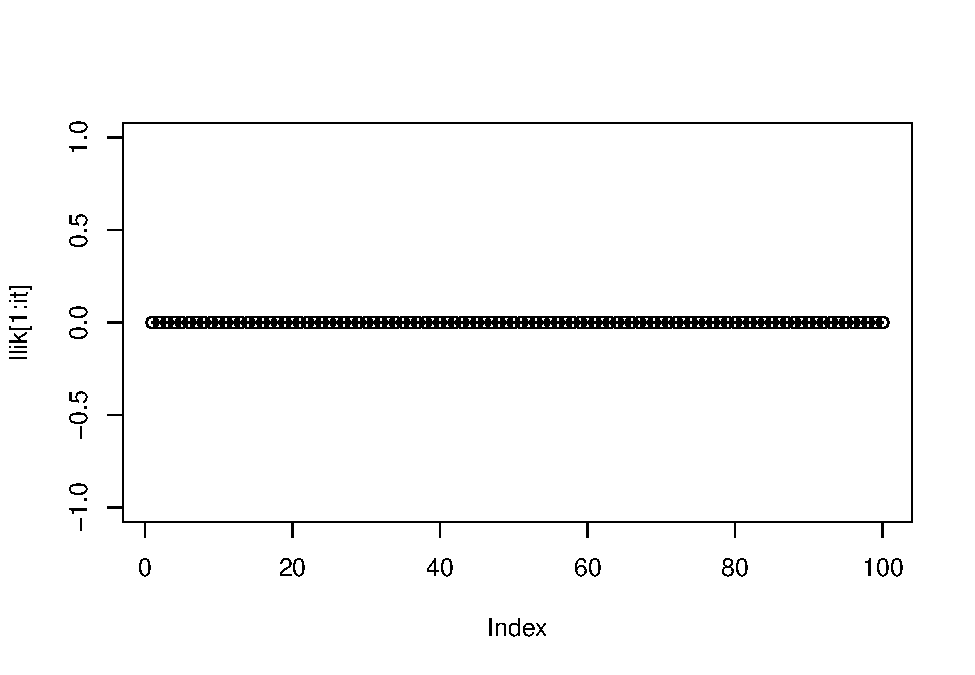
\includegraphics{Block2Lab1_files/figure-latex/2.1-3.pdf}

\hypertarget{appendix}{%
\section{Appendix}\label{appendix}}

\begin{lstlisting}[language=R]
knitr::opts_chunk$set(echo = TRUE)
library(randomForest)
x1<-runif(100)
x2<-runif(100)
trdata<-cbind(x1,x2)
y<-as.numeric(x1<x2)
trlabels<-as.factor(y)
set.seed(1234)
x1<-runif(1000)
x2<-runif(1000)
tedata<-cbind(x1,x2)
y<-as.numeric(x1<x2)
telabels<-as.factor(y)
plot(x1,x2,col=(y+1))

get_misc_err <- function(conf_mat){
  #Given a confusion matrix, return the misclassification error
  (sum(conf_mat)-sum(diag(conf_mat)))/sum(conf_mat)
}

r1 <- randomForest(trdata, trlabels, ntree = 1, nodesize = 25, keep.forest = TRUE)
p1 <- predict(r1, tedata)
conf_mat1 <- table(p1, telabels)
get_misc_err(conf_mat1)
cat("Mean misclassification error for 1 tree:", get_misc_err(conf_mat1), "\n")

r10 <- randomForest(trdata, trlabels, ntree = 10, nodesize = 25, keep.forest = TRUE)
p10 <- predict(r10, tedata)
conf_mat10 <- table(p10, telabels)
get_misc_err(conf_mat10)
cat("Mean misclassification error for 10 trees:", get_misc_err(conf_mat10), "\n")

r100 <- randomForest(trdata, trlabels, ntree = 100, nodesize = 25, keep.forest = TRUE)
p100 <- predict(r100, tedata)
conf_mat100 <- table(p100, telabels)
get_misc_err(conf_mat100)
cat("Mean misclassification error for 100 trees:", get_misc_err(conf_mat100), "\n")



get_training <- function(){
  x1<-runif(100)
  x2<-runif(100)
  trdata<-cbind(x1,x2)
  y<-as.numeric(x1<x2)
  trlabels<-as.factor(y)
  return(list(trdata, trlabels))
}
meR1 <- c()

meR10 <- c()

meR100 <- c()

for(i in 1:1000){
  
  #cat("Iteration:", i, "\r")
  #Creating the training data
  training <- get_training()
  trdata <- training[[1]]
  trlabels <- training[[2]]
  
  
  r1 <- randomForest(trdata, trlabels, ntree = 1, nodesize = 25, keep.forest = TRUE)
  p1 <- predict(r1, tedata)
  conf_mat1 <- table(p1, telabels)
  meR1 <- c(meR1, get_misc_err(conf_mat1))
  
  r10 <- randomForest(trdata, trlabels, ntree = 10, nodesize = 25, keep.forest = TRUE)
  p10 <- predict(r10, tedata)
  conf_mat10 <- table(p10, telabels)
  meR10 <- c(meR10, get_misc_err(conf_mat10))
  
  r100 <- randomForest(trdata, trlabels, ntree = 100, nodesize = 25, keep.forest = TRUE)
  p100 <- predict(r100, tedata)
  conf_mat100 <- table(p100, telabels)
  meR100 <- c(meR100, get_misc_err(conf_mat100))
}

#Overall mean
cat("Overall mean for 1 tree:", mean(meR1), "\n")
cat("Overall variance for 1 tree:", var(meR1), "\n")
cat("Overall mean for 10 trees:", mean(meR10), "\n")
cat("Overall variance for 10 trees:", var(meR10), "\n")
cat("Overall mean for 100 trees:", mean(meR100), "\n")
cat("Overall variance for 100 trees:", var(meR100), "\n")

set.seed(1234)
x1<-runif(1000)
x2<-runif(1000)
tedata<-cbind(x1,x2)
y<-as.numeric(x1<0.5)
telabels<-as.factor(y)
plot(x1,x2,col=(y+1))

get_training <- function(){
  x1<-runif(100)
  x2<-runif(100)
  trdata<-cbind(x1,x2)
  y<-as.numeric(x1<0.5)
  trlabels<-as.factor(y)
  return(list(trdata, trlabels))
}
meR1 <- c()

meR10 <- c()

meR100 <- c()

for(i in 1:1000){
  
  #cat("Iteration:", i, "\r")
  #Creating the training data
  training <- get_training()
  trdata <- training[[1]]
  trlabels <- training[[2]]
  
  
  r1 <- randomForest(trdata, trlabels, ntree = 1, nodesize = 25, keep.forest = TRUE)
  p1 <- predict(r1, tedata)
  conf_mat1 <- table(p1, telabels)
  meR1 <- c(meR1, get_misc_err(conf_mat1))
  
  r10 <- randomForest(trdata, trlabels, ntree = 10, nodesize = 25, keep.forest = TRUE)
  p10 <- predict(r10, tedata)
  conf_mat10 <- table(p10, telabels)
  meR10 <- c(meR10, get_misc_err(conf_mat10))
  
  r100 <- randomForest(trdata, trlabels, ntree = 100, nodesize = 25, keep.forest = TRUE)
  p100 <- predict(r100, tedata)
  conf_mat100 <- table(p100, telabels)
  meR100 <- c(meR100, get_misc_err(conf_mat100))
}

#Overall mean
cat("Overall mean for 1 tree:", mean(meR1), "\n")
cat("Overall variance for 1 tree:", var(meR1), "\n")
cat("Overall mean for 10 trees:", mean(meR10), "\n")
cat("Overall variance for 10 trees:", var(meR10), "\n")
cat("Overall mean for 100 trees:", mean(meR100), "\n")
cat("Overall variance for 100 trees:", var(meR100), "\n")
set.seed(1234)
x1<-runif(1000)
x2<-runif(1000)
tedata<-cbind(x1,x2)
y<-as.numeric(((x1<0.5 & x2<0.5) | (x1>0.5 & x2>0.5)))
telabels<-as.factor(y)
plot(x1,x2,col=(y+1))

get_training <- function(){
  x1<-runif(100)
  x2<-runif(100)
  trdata<-cbind(x1,x2)
  y<-as.numeric((x1<0.5 & x2<0.5) | (x1>0.5 & x2>0.5))
  trlabels<-as.factor(y)
  return(list(trdata, trlabels))
}
meR1 <- c()

meR10 <- c()

meR100 <- c()

for(i in 1:1000){
  
  #cat("Iteration:", i, "\r")
  #Creating the training data
  training <- get_training()
  trdata <- training[[1]]
  trlabels <- training[[2]]
  
  
  r1 <- randomForest(trdata, trlabels, ntree = 1, nodesize = 12, keep.forest = TRUE)
  p1 <- predict(r1, tedata)
  conf_mat1 <- table(p1, telabels)
  meR1 <- c(meR1, get_misc_err(conf_mat1))
  
  r10 <- randomForest(trdata, trlabels, ntree = 10, nodesize = 12, keep.forest = TRUE)
  p10 <- predict(r10, tedata)
  conf_mat10 <- table(p10, telabels)
  meR10 <- c(meR10, get_misc_err(conf_mat10))
  
  r100 <- randomForest(trdata, trlabels, ntree = 100, nodesize = 12, keep.forest = TRUE)
  p100 <- predict(r100, tedata)
  conf_mat100 <- table(p100, telabels)
  meR100 <- c(meR100, get_misc_err(conf_mat100))
}

#Overall mean
cat("Overall mean for 1 tree:", mean(meR1), "\n")
cat("Overall variance for 1 tree:", var(meR1), "\n")
cat("Overall mean for 10 trees:", mean(meR10), "\n")
cat("Overall variance for 10 trees:", var(meR10), "\n")
cat("Overall mean for 100 trees:", mean(meR100), "\n")
cat("Overall variance for 100 trees:", var(meR100), "\n")
set.seed(1234567890)
max_it <- 100 # max number of EM iterations
min_change <- 0.1 # min change in log lik between two consecutive iterations
n=1000 # number of training points
D=10 # number of dimensions
x <- matrix(nrow=n, ncol=D) # training data
true_pi <- vector(length = 3) # true mixing coefficients
true_mu <- matrix(nrow=3, ncol=D) # true conditional distributions
true_pi=c(1/3, 1/3, 1/3)
true_mu[1,]=c(0.5,0.6,0.4,0.7,0.3,0.8,0.2,0.9,0.1,1)
true_mu[2,]=c(0.5,0.4,0.6,0.3,0.7,0.2,0.8,0.1,0.9,0)
true_mu[3,]=c(0.5,0.5,0.5,0.5,0.5,0.5,0.5,0.5,0.5,0.5)
plot(true_mu[1,], type="o", col="blue", ylim=c(0,1))
points(true_mu[2,], type="o", col="red")
points(true_mu[3,], type="o", col="green")
# Producing the training data
for(i in 1:n){
  m <- sample(1:3,1,prob=true_pi)
  for(d in 1:D){
    x[i,d] <- rbinom(1,1,true_mu[m,d])
  }
}
M=3 # number of clusters
w <- matrix(nrow=n, ncol=M) # weights
pi <- vector(length = M) # mixing coefficients
mu <- matrix(nrow=M, ncol=D) # conditional distributions
llik <- vector(length = max_it) # log likelihood of the EM iterations
# Random initialization of the parameters
pi <- runif(M,0.49,0.51)
pi <- pi / sum(pi)
for(m in 1:M){
  mu[m,] <- runif(D,0.49,0.51)
}
pi
mu
for(it in 1:max_it) {
  plot(mu[1,], type="o", col="blue", ylim=c(0,1))
  points(mu[2,], type="o", col="red")
  points(mu[3,], type="o", col="green")
  #points(mu[4,], type="o", col="yellow")
  Sys.sleep(0.1)
  # E-step: Computation of the weights
  # Your code here
  #Log likelihood computation.
  # Your code here
  cat("iteration: ", it, "log likelihood: ", llik[it], "\n")
  flush.console()
  # Stop if the lok likelihood has not changed significantly
  # Your code here
  #M-step: ML parameter estimation from the data and weights
  # Your code here
}
pi
mu
plot(llik[1:it], type="o")
\end{lstlisting}


\end{document}
